\documentclass[oneside, openany]{tufte-book}

\usepackage[]{lipsum}
\usepackage{circuitikz}
\usepackage{enumitem}
\usepackage[dvipsnames]{xcolor}
\usepackage{tcolorbox}
\usepackage{listings}
\setcounter{tocdepth}{1}
\usepackage{booktabs}
\usepackage{amsmath, xparse}
\usepackage{parskip}
\usepackage[font={color=black}]{caption}
\captionsetup{
	font={footnotesize}
}

\geometry{
	paperwidth=640pt,
	paperheight=480pt,
	right=7cm, left=25mm, bottom=25mm
}

\titlespacing*{name=\chapter,numberless}{0pt}{-35pt}{40pt}
\titlespacing*{name=\chapter}{0pt}{-22pt}{40pt}
\titleformat{\part}[block]{\normalfont\Huge\filcenter\color{darkgray}}{\partname\ \thepart}{2em}{} % Adjust the format as needed


\renewcommand{\maketitlepage}{%
{
		\begin{fullwidth}%
			\thispagestyle{empty}
			\fontsize{18}{20}\selectfont\par\noindent\textcolor{darkgray}{\itshape\thanklessauthor}%
			\vspace{11.5pc}%
			\fontsize{36}{40}\selectfont\par\noindent\textcolor{darkgray}{\thanklesstitle}%
			\vspace{2mm}
			\fontsize{14}{16}\selectfont\par\noindent\textcolor{darkgray}{\scshape\thanklesspublisher}%
		\end{fullwidth}%
}
}

\AtBeginDocument{\setlength{\parindent}{0cm}}

\newcommand{\preface}{
\newpage
\section*{Preface}
The purpose of this document is to act as a comprehensive note for my understanding on the subject matter. I may also use references aside from the lecture material to further develop my understanding, and these references will be listed here. 

This document should eventually serve as a standalone reference for learning or review of the subject matter. There is also a lot of organization within these documents, please refer to the table of contents within your PDF viewer for ease of navigation.

\section*{References}
\begin{itemize}
	\myreferences
\end{itemize}
}


%% NEEDS TO BE DEFINED IN MAIN DOC
% define title, author, publisher, and \def\myreferences for use in the preface

\let\cleardoublepage\clearpage

%%% -------------------
%%% |  CUSTOM COLORS  |
%%% -------------------

\definecolor{whitesmoke}{HTML}{CCCCCC}
\definecolor{grey}{HTML}{686E75}
\definecolor{red}{HTML}{D65B5C}
\definecolor{orange}{HTML}{EF8511}
\definecolor{yellow}{HTML}{D3B006}
\definecolor{green}{HTML}{5DB267}
\definecolor{blue}{HTML}{62ABF3}
\definecolor{purple}{HTML}{7F76DA}
\definecolor{pink}{HTML}{B76CC7}
\definecolor{greyblue}{HTML}{171B20} % default: 171B20

%%% -------------------
%%% | CUSTOM COMMANDS |
%%% -------------------


%----------------------------------------------------------------------------------------
%   HIGHLIGHT ENVIRONMENT
%----------------------------------------------------------------------------------------

\newtcolorbox{highlight}{
	colback=greyblue,
	colframe=whitesmoke,
	coltext=whitesmoke,
	boxrule=0.75pt,
	boxsep=4pt,
	arc=0pt,
	outer arc=0pt,
	enlarge bottom by=0.25cm,
	enlarge top by=0.15cm
}

%----------------------------------------------------------------------------------------
%   REMARK ENVIRONMENT
%----------------------------------------------------------------------------------------

\newtcolorbox{remark}{
	colback=greyblue,
	colframe=whitesmoke,
	coltext=whitesmoke,
	boxrule=0pt,
	leftrule=0.75pt,
	boxsep=4pt,
	arc=0pt,
	outer arc=0pt,
	enlarge bottom by=0.5cm,
}

%----------------------------------------------------------------------------------------
%   OUTLINE ENVIRONMENT
%----------------------------------------------------------------------------------------

\newtcolorbox{outline}[1][4pt]{
	enhanced,
	colback=greyblue,
	colframe=greyblue, % To essentially hide the frame, but we will draw the corners manually
	coltext=whitesmoke,
	boxrule=1pt,
	boxsep=#1,
	arc=1pt,
	outer arc=1pt,
	enlarge bottom by=0.5cm,
	overlay={
		% Top left corner
		\draw[whitesmoke,line width=1pt] 
		(frame.north west) -- ++(0,-0.25*\tcbtextheight)
		(frame.north west) -- ++(0.25*\tcbtextwidth,0);
		% Bottom right corner
		\draw[whitesmoke,line width=1pt]
		(frame.south east) -- ++(0,0.25*\tcbtextheight)
		(frame.south east) -- ++(-0.25*\tcbtextwidth,0);
	}
}

%----------------------------------------------------------------------------------------
%   LSTLISTING ENVIRONMENT
%----------------------------------------------------------------------------------------
\lstset
{ %Formatting for code in appendix
	language=Verilog,
	frame=single,
	basicstyle=\footnotesize\texttt,
	numbers=left,
	stepnumber=1,
	showstringspaces=false,
	tabsize=4,
	breaklines=true,
	breakatwhitespace=false,
	aboveskip=2em,
	belowcaptionskip=0.75em
}
\renewcommand{\lstlistingname}{\color{black} Code Snippet}
\lstset{ %
	basicstyle=\footnotesize\ttfamily,        % size of fonts used for the code
	breaklines=true,                 % automatic line breaking only at whitespace
	captionpos=b,                    % sets the caption-position to bottom
	commentstyle=\color{grey},    % comment style
	escapeinside={\%*}{*)},          % if you want to add LaTeX within your code
	keywordstyle=\color{blue!55!green},       % keyword style
	stringstyle=\color{green!75!white},     % string literal style
}

%----------------------------------------------------------------------------------------
%   DEFINITION + THEORY ENVIRONMENT
%----------------------------------------------------------------------------------------
\newenvironment{definition}{
	\begin{itemize}[labelindent=5em,labelsep=0.25cm,leftmargin=*]
		\item[{{\itshape\scshape\color{purple!55!red}{Definition}}}]{}
	}
	{
	\end{itemize}
}


\newenvironment{theory}{
	\begin{itemize}[labelindent=4.2em,labelsep=0.5cm,leftmargin=*]
		\item[{{\itshape\scshape\color{red!55!purple}{Theorem}}}]
	}
	{
	\end{itemize}
}

\newenvironment{bullets}{
	\begin{itemize}[leftmargin=2em]
	}
	{
	\end{itemize}
}
%----------------------------------------------------------------------------------------
%   KEYWORD, CODE, EMPH & STROKE ENVIRONMENT
%----------------------------------------------------------------------------------------
\newcommand{\keyword}[1]{{{\bfseries\color{purple}{#1}\,}}}
\newcommand{\code}[1]{{\ttfamily\color{blue!55!green}\,{#1}\,}}
\newcommand{\str}[1]{{\ttfamily\color{green!55!white}\,{"#1"}\,}}
\renewcommand{\emph}[1]{{\itshape#1}} % renew emph style here as required
% END_FOLD ENVIRONMENTS
 % preamble
\lstset{language=C}

\title{Data Engineering \\ \& Machine Learning}
\author{Arnav Goyal}
\publisher{Winter 2024 / AISE 3010}

\tikzstyle{node} = [draw=darkgray, rectangle, fill=darkgray, text=darkgray]
\tikzstyle{myarrow} = [
>=Stealth,
node distance=1.5cm,
auto,
myarrow/.style={
	decoration={
		markings,
		mark=at position 0.5 with {\arrow{Stealth}}
	},
	postaction={decorate}
}
]
\usetikzlibrary{positioning, arrows.meta, decorations.markings, decorations.pathreplacing}

\def\myreferences{
	\item Provided Course Material \& Lecture Notes
	\item Neural Networks and Learning Machines - 3e - S. Haykin
}

\begin{document}
	\frontmatter
	\pagenumbering{roman}
	\maketitle
	\preface
	
	\mainmatter
	\pagenumbering{arabic}

	\chapter{The Perceptron}

In this chapter we will be going over the architecture of the most basic \keyword{neural network (NN)}, called the \keyword{perceptron}\sidenote{Also called Rosenblatt's perceptron}. 

\section{The Neuron}

The most basic unit of a perceptron is called the \keyword{neuron}\sidenote{More specifically, the McCulloch-Pitts model of a neuron}. The structure of a neuron can be seen in Figure \ref{neuron}, each neuron possesses the following.
\begin{bullets}
	\item Some \keyword{input features} $x_1\,\ldots\,x_n$
	\item A corresponding \keyword{weight} for each feature $w_1\,\ldots\,w_n$
	\item A \keyword{bias} $b$
	\item An \keyword{activation function} $\varphi(.)$
	\item An \keyword{output} $y$
\end{bullets}

\begin{marginfigure}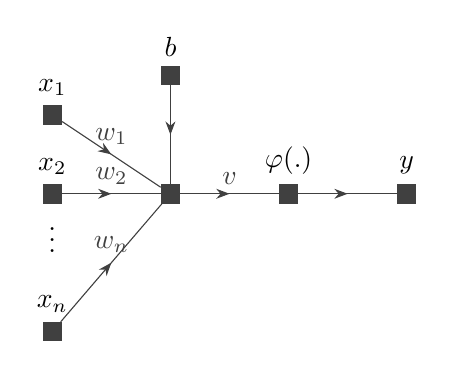
\begin{tikzpicture}[>=Stealth, node distance=1.5cm, auto, myarrow]
	
	% Inputs
	\node[node, label=$x_1$, node distance=1cm] (inputa) {};
	\node[node, label=$x_2$, below of=inputa, node distance=1cm] (inputb) {};
	\node[label=$\vdots$, below of=inputb, node distance=1cm] (dots) {};
	\node[node, label=$x_n$, below of=dots, node distance=0.75cm] (inputc) {};
	
	% sum, bias and activation
	\node [node, right of = inputb] (sum) {};
	\node[node, above of = sum, label=$b$] (bias) {};
	\node[node, right of = sum, label=$\varphi(.)$] (activation) {};
	
	% output
	\node [node, right of = activation, label=$y$] (output) {};
	
	% connections
	\draw [myarrow, darkgray] (inputa) -- (sum) node[midway, above] {$w_1$};
	\draw [myarrow, darkgray] (inputb) -- (sum) node[midway, above] {$w_2$};
	\draw [myarrow, darkgray] (inputc) -- (sum) node[midway, above] {$w_n$};
	\draw [myarrow, darkgray] (bias) -- (sum); 
	\draw [myarrow, darkgray] (sum) -- (activation) node[midway, above] {$v$};
	\draw [myarrow, darkgray] (activation) -- (output);
	
\end{tikzpicture} \centering \caption{Signal Flow Graph of A Neuron} \label{neuron}  \end{marginfigure}

A neuron essentially performs the following operation, which can be seen from the signal flow graph.
\[ y = \varphi \left( \sum_{i=1}^{n} w_i x_i + b \right)\]

\section{The Basic Perceptron}

The perceptron was initially built with just a single neuron, and was limited to performing \keyword{binary classification} or \keyword{linear regression.}
\begin{bullets}
	\item In binary classification, each training sample $(X,y)$ contains some data $X=x_1 , x_2, \ldots$ and a label $y\in\left\{ -1, +1 \right\}$
	\item In linear regression the dependent variable is $y\in\mathbb{R}$
\end{bullets}
Overall, the perceptron was created to deal with binary classification problems.
\begin{bullets}
	\item This means that both classes $c_1$ and $c_2$ need to be \keyword{linearly seperable}\sidenote{We need to be able to draw a hyperplane that clearly seperates every instances from both classes, such that only instances from the same class are on a distinct side of the hyperplane}
	\item The perceptron is essentially trying to find a \keyword{linear separator} between the two classes\sidenote{Given that the activation function, $\varphi(.) \leftarrow \text{sgn}(.) $}, such that $\sum w_i x_i + b = 0$.
\end{bullets}

\section{Multi-Layered Perceptrons}

The most basic perceptron was basically a single-layered NN, but now we will discuss the \keyword{multi-layered perceptron (MLP)} which uses more layers, with possibly more neurons in each layer\sidenote{We do this to overcome the perceptrons practical limitations}.

Before I continue, lets clarify some terminology.
\begin{bullets}
	\item The \keyword{input layer} is the first layer with neurons that each accept 1 feature. In total, an input layer with $k$ neurons can accept $k$ features. 
	\item The \keyword{output layer} is the last layer, containing neurons that spit out one output each. In total an output layer with $h$ neurons produces an output with dimensionality of $h$.
	\item The \keyword{hidden layers} are the other layers sandwiched in between the input and output. When we say a "an $n$-layered network", we are referring to the amount of hidden layers in the network.
\end{bullets}
This is illustrated in Figure \ref{layers}.

\begin{marginfigure} \centering \caption{Layers in an MLP} \label{layers} 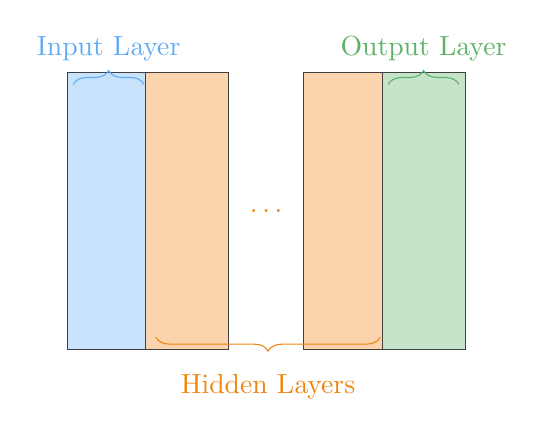
\begin{tikzpicture}[draw=darkgray]
	%diagram
	\node[draw, rectangle, minimum height=10em, minimum width=3em, fill=blue!35] (input) {};
	\node[draw, rectangle, minimum height=10em, right of = input, minimum width=3em, fill=orange!35] (hidden1) {};
	\node[right of = hidden1, text=orange] (dots) {$\ldots$};
	\node[draw, rectangle, minimum height=10em, right of = dots, minimum width=3em, fill=orange!35] (hidden2) {};
	\node[draw, rectangle, minimum height=10em, right of = hidden2, minimum width=3em, fill=green!35] (output) {};
	
	%labels
	\draw [blue,decorate, decoration={brace,amplitude=5pt, raise=4ex}] (-0.45,1) -- (0.45,1) node[midway, yshift=3em, text=blue] {Input Layer};
	\draw [green, text=green, decorate, decoration={brace,amplitude=5pt, raise=4ex}] (3.55,1)-- (4.45,1) node[midway, yshift=3em] {Output Layer};
	\draw [orange, text=orange, decorate, decoration={brace,amplitude=5pt, mirror, raise=4ex}] (0.6,-1) -- (3.45,-1) node[midway, yshift=-3.5em] {Hidden Layers};
\end{tikzpicture} \end{marginfigure}

In order to construct a MLP we must ensure the following.
\begin{bullets}
	\item The activation function $\varphi_i (.)$ of each neuron $i$ is a \keyword{differentiable} and non-linear function.
	\item The network contains at least one layer that is \keyword{hidden} from the input and output nodes (hidden layers).
	\item The network exhibits a high degree of \keyword{connectivity} through synaptic weights of the network.
\end{bullets}
These conditions ensure that the network becomes complex, but also so complex that we struggle to understand the behavior of the network.

\section{Batch \& Iterative Learning}

As we work our way up to understanding the training of the MLP we should account for the two methods of teaching the MLP, called \keyword{batch learning} and \keyword{iterative learning}\sidenote{In the textbook this is called \emph{on-line learning} but this was obviously confusing so I changed it for this note.}
\begin{bullets}
	\item Batch learning consists of presenting a batch of training examples to the network at the same time
	\item Iterative learning consists of presenting one training example to the network at a time.
\end{bullets}

Batch learning has the advantages of  providing an accurate-estimation of the gradient vector, and allowing a parallelization of the learning process. While iterative learning is simple to implement and can utilize redundancies in the dataset.

	\chapter{Backpropagation}

Now we are going to dive into the complex algorithm called \keyword{backpropagation} which is the way modern NNs are trained. There are two cases for this algorithm
\begin{bullets}
	\item When a neuron is an output neuron
	\item When a neuron isn't an output neuron
\end{bullets}
We will be starting with the former, but be warned! this is going to be a painful and math-intensive chapter.

\begin{marginfigure}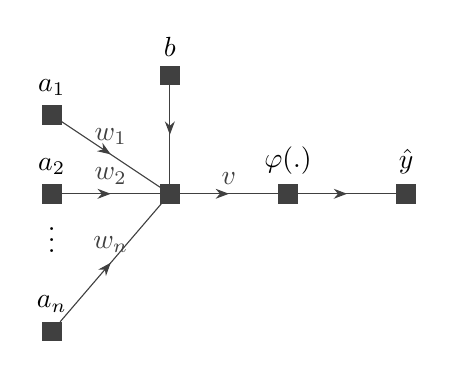
\begin{tikzpicture}[>=Stealth, node distance=1.5cm, auto, myarrow]
		
		% Inputs
		\node[node, label=$a_1$, node distance=1cm] (inputa) {};
		\node[node, label=$a_2$, below of=inputa, node distance=1cm] (inputb) {};
		\node[label=$\vdots$, below of=inputb, node distance=1cm] (dots) {};
		\node[node, label=$a_n$, below of=dots, node distance=0.75cm] (inputc) {};
		
		% sum, bias and activation
		\node [node, right of = inputb] (sum) {};
		\node[node, above of = sum, label=$b$] (bias) {};
		\node[node, right of = sum, label=$\varphi(.)$] (activation) {};
		
		% output
		\node [node, right of = activation, label=$\hat y$] (output) {};
		
		% connections
		\draw [myarrow, darkgray] (inputa) -- (sum) node[midway, above] {$w_1$};
		\draw [myarrow, darkgray] (inputb) -- (sum) node[midway, above] {$w_2$};
		\draw [myarrow, darkgray] (inputc) -- (sum) node[midway, above] {$w_n$};
		\draw [myarrow, darkgray] (bias) -- (sum); 
		\draw [myarrow, darkgray] (sum) -- (activation) node[midway, above] {$v$};
		\draw [myarrow, darkgray] (activation) -- (output);
		
	\end{tikzpicture} \centering \caption{An Output Neuron} \label{outputneuron}  \end{marginfigure}


\section{The Error \& Cost Function}

Consider a neuron $j$ that is located in the output layer of an MLP. It has internal structure as shown by Figure \ref{outputneuron}. We also define the \keyword{error} $\varepsilon$, that gives a measure of how far our current output $\hat{y}$, is from our desired output $y$. For the purposes of this chapter:
\[  \varepsilon =  y - \hat{y}\]

We should also define a \keyword{cost function} $\ell$ as the \keyword{total error energy} of the whole network.\sidenote{This is usually defined at some iteration $n$ but this is left out for brevity.}
\[  \ell  = \frac{1}{2}\varepsilon^2 \]	

\section{The Output Neuron}

We are concerned with finding out how the loss function $\ell$ changes with respect to a certain weight $w_k$. In other words we are tasked with finding the derivative.\sidenote{We are tasked with finding  $\dfrac{\partial\ell}{\partial w_k}$}. We can do this through the \keyword{chain rule}.

\[	\frac{\partial\ell}{\partial w_k} = \frac{\partial \ell}{\partial \varepsilon}\cdot\frac{\partial\varepsilon}{\partial\hat{y}}\cdot\frac{\partial\hat{y}}{\partial w_k}\]

We can break down this derivative even further using Figure \ref{outputneuron}, resulting in Equation \ref{eq:1}. We can even extend this to see how we can change the biases, which is given in Equation \ref{eq:2}.

\begin{equation}
	\label{eq:1}
	\frac{\partial\ell}{\partial w_k} = \frac{\partial \ell}{\partial \varepsilon}\cdot\frac{\partial\varepsilon}{\partial\hat{y}}\cdot\frac{\partial\hat{y}}{\partial v}\cdot\frac{\partial v}{\partial w_k}
\end{equation}

\begin{equation}
	\label{eq:2}
	\frac{\partial\ell}{\partial b_k} = \frac{\partial \ell}{\partial \varepsilon}\cdot\frac{\partial\varepsilon}{\partial\hat{y}}\cdot\frac{\partial\hat{y}}{\partial v}\cdot\frac{\partial v}{\partial b_k}
\end{equation}

Analytically solving Equation \ref{eq:1} gives the following result:
	\[ \frac{\partial\ell}{\partial w_k} = -\varepsilon a_k \varphi'(v)	\]
	
\section{A Hidden Neuron}

When a neuron $j$ is located within a hidden layer of the MLP, there is no desired response for that neuron, accordingly the error signal for that neuron would have to be determined recursively, and work backwards from all neurons to where the neuron $j$ is located\sidenote{This is where the term \emph{backpropagation} comes from}.


\end{document}